
%%%%%%%%%%%%%%%%%%%%%%%%%%%%%%%%%%%%%%%%%%%%%%%%%%%%%%%%%%%%%%%%%%%%%%%%%%%%%%%%%%%%%%%%%%%%%%%%%%%%%%%%%%%%%%%%%%%%%%%%%%%%%%%%%%%%%%%%%%%%%%%%%%%%%%%%%%%%%%%%%%%%
\chapter{Importing data in Ondex}
\label{cha:import}
%%%%%%%%%%%%%%%%%%%%%%%%%%%%%%%%%%%%%%%%%%%%%%%%%%%%%%%%%%%%%%%%%%%%%%%%%%%%%%%%%%
Various ``parsers'' allow users to import data and convert it to OXL format (Ondex eXchange Language).
This format of data can then be used by Ondex mapping methods, transformers, etc.
or can simply be open in the Ondex front-end.

%%%%%%%%%%%%%%%%%%%%%%%%%%%%%%%%%%%%%%%%%%%%%%%%%%%%%%%%%%%%%%%%%%%%%%%%%%%%%%%%%%

\section{OXL Parser}
Parser for OXL files.

\begin{itemize}
  \item{IgnoreAttribute}\\
  Do not parse Attribute attributes with specified AttributeName
  \item{InputFile}\\
  OXL file to load
\end{itemize}
    
%%%%%%%%%%%%%%%%%%%%%%%%%%%%%%%%%%%%%%%%%%%%%%%%%%%%%%%%%%%%%%%%%%%%%%%%%%%%%%%%%%    
\section{Aracyc2 (Release 6, October 14, 2009)}

Download the Aracyc flatfile database from \url{http://www.plantcyc.org/downloads/license_agreement.faces}
(\url{ftp://ftp.arabidopsis.org/home/tair/home/tair/tmp/private/plantcyc/aracyc.tar.gz}).
Extract contents of the data directory inside the tar to the root directory (this includes .col and .dat files).
\begin{itemize}
  \item{InputDir}\\
  Absolute path to input directory
\end{itemize}
    
%%%%%%%%%%%%%%%%%%%%%%%%%%%%%%%%%%%%%%%%%%%%%%%%%%%%%%%%%%%%%%%%%%%%%%%%%%%%%%%%%%    
\section{AtRegNet Parser (Expanded version)}
Parses AtRegNet ({\it{Arabidopsis thaliana}} Regulatory Networks) focussing on protein protein interactions.
This requires AtRegNet\_(some date).zip. Getting a hold of this file requires registering with AGRIS (\url{http://arabidopsis.med.ohio-state.edu/downloads.html}).
This zip file then needs to be decompressed to give a .tbl (the corresponding .txt file is not read by the parser) 
which must be placed within the data directory in the Ondex folder hierarchy (specified by -Dondex.dir).

\begin{itemize}
  \item{InputFile}\\
  Absolute path to input file
\end{itemize}
    
%%%%%%%%%%%%%%%%%%%%%%%%%%%%%%%%%%%%%%%%%%%%%%%%%%%%%%%%%%%%%%%%%%%%%%%%%%%%%%%%%%     
\section{AtRegNet Parser (Simple version)}
General parsing of AtRegNet ({\it{Arabidopsis thaliana}} Regulatory Networks).
This requires AtRegNet\_(some date).zip, AtcisDB.zip, and AtTFDB.zip.
Getting a hold of this file requires registering with AGRIS (\url{http://arabidopsis.med.ohio-state.edu/downloads.html}).

The following zip files need to have the following files unpacked to the same folder. Specifically, the following files are required:
\begin{itemize}
  \item reg\_net\_(some date).tbl from AtRegNet\_(some date).zip
  \item GeneInfo.tbl from AtcisDB.zip
  \item families\_data.tbl from from AtTFDB.zip
  \item families\_pep.tbl from AtTFDB.zip
\end{itemize}

The file reg\_net\_(some date).tbl will need to be renamed to reg\_net.tbl
\begin{itemize}
  \item{InputDir}\\
  Absolute path to input directory
\end{itemize}
   
%%%%%%%%%%%%%%%%%%%%%%%%%%%%%%%%%%%%%%%%%%%%%%%%%%%%%%%%%%%%%%%%%%%%%%%%%%%%%%%%%%     
\section{BioCyc BioPAX parser (BioPax version 2)}   
The BioCyc (\url{http://biocyc.org/intro.shtml}) parser is a generic parser. 
Beside the import data directory it requires two arguments, one for DataSource ({\it{e.g.}}, SolCyc) 
and one for TaxId (the NCBI organism identifier, {\it{e.g.}}, 3702 for {\it{A.thaliana}}).

The BioCyc parser only parses the very basic set of features from a BioCyc database. 
That is why there are more specific parser like AraCyc, 
which parse more accessions and adapt to the notions of the curators used for not clearly structured data.

BioCyc databases are usually organism specific, {\it{i.e.}} you would be downloading the flat files per organism anyway, 
{\it{e.g.}}, one for SolCyc, one for LycoCyc and so on however they might be called. 
Therefore to import multiple organism you simply call the parser multiple times, 
at each time pointing to the respective directory of the organism specific BioCyc database.    
    
The parser takes a biopax.owl file (not a .gzip).
It also needs a translation file that specifies the translation of the Ondex represenation 
that should be placed in the same directory as the data being parsed.
This file is included in the core data directory.    

\begin{itemize}
  \item{TaxId}\\
  Which taxonomy id should be assigned to the database entries.
  \item{DataSource}\\
  The source of the database, to disinguish different databases, e.g. MC = MetaCyc, AC=AraCyc
  \item{InputFile}\\
  Absolute path to input file
\end{itemize}


%%%%%%%%%%%%%%%%%%%%%%%%%%%%%%%%%%%%%%%%%%%%%%%%%%%%%%%%%%%%%%%%%%%%%%%%%%%%%%%%%%     
\section{BioGrid}
Parses the BioGRID (General Repository for Interaction Datasets) database flatfiles.
It creates an interaction concept for each interaction in the file. 
Each interaction concept is connected to an active participant and a passive participant, 
as well as to a publication that documents it.
The parser automatically recognizes whether the interaction is a genetic or physical interaction 
and what subclass of interaction it is. It then sets the interaction's class and the 
participants' classes accordingly. Genetic interactions have 'Gene' participants, 
physical interactions have 'Polypeptide' participants.
Download from \url{http://www.thebiogrid.org/downloads.php}.

\begin{itemize}
  \item{InputFile}\\
  Absolute path to input file
  \item{TranslationFile}\\
  Absolute path to the desired translation file
  \item{TaxIDRestriction}\\
  Taxonomy ID restriction. Only genes/proteins of the given taxa will be considered. If empty, all will be considered.
\end{itemize}
    
%%%%%%%%%%%%%%%%%%%%%%%%%%%%%%%%%%%%%%%%%%%%%%%%%%%%%%%%%%%%%%%%%%%%%%%%%%%%%%%%%%     
\section{BRENDA Parser (July 2009)}
Parser for the BRENDA database (comprehensive enzyme information system). 
Download from \url{http://www.brenda-enzymes.info/} (download link in the left hand side menu).
\begin{itemize}
  \item{Species}\\
  Species taxonomy identifier from NCBI preferred.
  \item{InputDir}\\
  Absolute path to input directory
\end{itemize}
    
%%%%%%%%%%%%%%%%%%%%%%%%%%%%%%%%%%%%%%%%%%%%%%%%%%%%%%%%%%%%%%%%%%%%%%%%%%%%%%%%%%    
%\section{Coex}
%Parser for coexpression databases. Download data from \url{http://coxpresdb.jp/} or \url{http://atted.jp/}.
%\begin{itemize}
%\item{RelationType}\\
%Specify which existing relations to add correlation score to.
%\item{Rank}\\
%Rank cut-off.
%\item{Filter\_file}\\
%Accessions of stable ges to be excluded, one accession per line.
%\item{Threshold}\\
%Correlation strength cut-off.
%\item{Accession}\\
%Accession used by the coexpression database to identify entries.
%\item{Random\_nodes}\\
%Number of random nodes in the network.
%\item{Random\_edges}\\
%Number of random edges in the network.
%\item{Input folder}\\
%Folder with data to import.
%\end{itemize}
    
%%%%%%%%%%%%%%%%%%%%%%%%%%%%%%%%%%%%%%%%%%%%%%%%%%%%%%%%%%%%%%%%%%%%%%%%%%%%%%%%%%    
\section{Correlation table parser}
A relation centric aproach to importing concepts and relations Concepts are defined as a header list. 
Relations are defined in value matrix/s where the values are added as a Attribute property on the relation. 
Where no attributes are specified no relation is created. Multiple values may be assigned by the use of additional matrices.
For example, 
\begin{itemize}
  \item Table headers: gene names
  \item Matrix 1: correlation coefficients corresponding to the genes
  \item Matrix 2: p values 
\end{itemize}
NB: A restriction of this parser is that AttributeName objects
parsed in must be instantiatable with a single string as the constructor.
\begin{itemize}
  \item{HeaderValues}\\
  Header Values representing concepts in a list form (concept values will be added as unambiguous accessions).
  \item{InclusionList}\\
  Genes from the matrices to include (all other genes will be ignored).
  \item{HeaderConceptClass}\\
  The ConceptClass to assign to concepts
  \item{DataSource}\\
  DataSource to assign to these concepts and relations.
  \item{AccessionCV}\\
  The DataSource for the accession idetifying the headers.
  \item{EvidenceType}\\
  EvidenceType to assign to these concepts and relations.
  \item{HeaderAttributeName}\\
  An AttributeName and value to create as a Attribute on each Concept.
  \item{CorrelationAttributeName}\\
  Specify a correlation AttributeName.
  \item{CorrelationFile}\\
  Specify a CorrelationFile.
  \item{PValueCutOff}\\
  The highest P-value allowed.
  \item{MinCorrelation}\\
  The minimum correlation allowed, defined as values greater that the absoluted correlation value (parsed when the MinCorrelation $>$ abs(correlation)).
  \item{InputDir}\\
  Absolute path to input directory.
\end{itemize}
    
    
%%%%%%%%%%%%%%%%%%%%%%%%%%%%%%%%%%%%%%%%%%%%%%%%%%%%%%%%%%%%%%%%%%%%%%%%%%%%%%%%%%    
\section{Customtab}
Application specific tab-delimited file parser, not for general use.
\begin{itemize}
  \item{InputFile}\\
  Absolute path to input file
\end{itemize}
    
    
%%%%%%%%%%%%%%%%%%%%%%%%%%%%%%%%%%%%%%%%%%%%%%%%%%%%%%%%%%%%%%%%%%%%%%%%%%%%%%%%%%    
\section{Drastic}
Drastic (Database Resource for the Analysis of Signal Transduction In Cells) parser for the file: ``Drastic Data.csv''
from \url{http://www.scri.sari.ac.uk/TiPP/PPS/DRASTIC/mpage/downloads.asp}.
\begin{itemize}
  \item{InputFile}\\
  Absolute path to input file
\end{itemize}
    
    
%%%%%%%%%%%%%%%%%%%%%%%%%%%%%%%%%%%%%%%%%%%%%%%%%%%%%%%%%%%%%%%%%%%%%%%%%%%%%%%%%%    
\section{EXPASY ENZYME (4/10/2009)}
EC nomenclature parser for the files: ``enzclass.txt'', ``enzyme.dat''
from \url{ftp://ftp.expasy.org/databases/enzyme/release_with_updates/}.
\begin{itemize}
  \item{Deleted}\\
  This specifies whether the enzymes with a deleted flag will be parsed from the EC database.
  \item{InputDir}\\
  Absolute path to input directory.
\end{itemize}
    
    
%%%%%%%%%%%%%%%%%%%%%%%%%%%%%%%%%%%%%%%%%%%%%%%%%%%%%%%%%%%%%%%%%%%%%%%%%%%%%%%%%%    
\section{FASTA file parser}
\begin{itemize}
  \item{InputFile}\\
  Absolute path to input file
  \item{FastaFileType}\\
  This setting must be used in order to parse the fasta header as best as possible.
  The fasta file type ``simple'' is the most generic type.
  Other types are ``AFFYMETRIX'', ``NCBI'', ``gramene'' and ``custom''.
  \item{TaxId}\\
  Specify a taxonomy identifier (species).
  \item{CC}\\
  The type of sequences ({\it{e.g.}}, target, gene, protein).
  \item{DataSource}\\
  The source of the sequences ({\it{e.g.}}, AFFY, TAIR, dbEST, unknown).
  \item{POS\_TO\_ACCESSION}\\
  No description
  \item{SeqType}\\
  The type (attribute name) of the sequences ({\it{e.g.}}, ``NA'', ``AA'').
  \item{Separator}\\
  Regular expressions to split header in simple FASTA parser.
  \item{AccessionRegEx}\\
  Regular expressions to be used as an additional accession.
\end{itemize}
    
    
%%%%%%%%%%%%%%%%%%%%%%%%%%%%%%%%%%%%%%%%%%%%%%%%%%%%%%%%%%%%%%%%%%%%%%%%%%%%%%%%%%    
\section{GenericOBO (OBO 1.2)}
OBO Ontology parser.
\begin{itemize}
  \item{OboType}\\
  This setting must be used in order to parse the OBO file as best as possible.
  The fasta file type ``generic'' is the most generic type.
  Other types are ``GO'', ``PO'' and ``ChEBI''.
  \item{Obsoletes}\\
  This specifies whether OBO-concepts with the obsolete flag should be parsed.
  \item{InputFile}\\
  Absolute path to input file
\end{itemize}
    
    
%%%%%%%%%%%%%%%%%%%%%%%%%%%%%%%%%%%%%%%%%%%%%%%%%%%%%%%%%%%%%%%%%%%%%%%%%%%%%%%%%%    
\section{Generif}
Parser for the GeneRIF file.   
Download from \url{ftp://ftp.ncbi.nih.gov/gene/GeneRIF/generifs_basic.gz}
Creates relations from Genes to Publications and assigns the GeneRIFs to them.

\begin{itemize}
  \item{TaxId}\\
  Will parse genes with comma separated taxonomy identifiers specified here.
  \item{InputDir}\\
  Absolute path to input directory.
\end{itemize}
    
    
%%%%%%%%%%%%%%%%%%%%%%%%%%%%%%%%%%%%%%%%%%%%%%%%%%%%%%%%%%%%%%%%%%%%%%%%%%%%%%%%%%    
\section{GO (OBO 1.2)}
GO Ontology parser for the file: ``gene\_ontology\_edit.obo'' in OBO v1.2 format 
from \url{http://www.geneontology.org/ontology/gene_ontology_edit.obo} (latest tested version: 16/01/07).
\begin{itemize}
  \item{Obsoletes}\\
  This specifies whether OBO-concepts with the obsolete flag should be parsed.
  \item{IsGOSLIM}\\
  Parse GO in as GOSLIM
  \item{InputFile}\\
  Absolute path to input file
\end{itemize}
    
%%%%%%%%%%%%%%%%%%%%%%%%%%%%%%%%%%%%%%%%%%%%%%%%%%%%%%%%%%%%%%%%%%%%%%%%%%%%%%%%%%    
\section{GeneAnnotationFormat (GAF 1.0 and 2.0)}
Gene Annotation File Format Guide: \url{http://geneontology.org/GO.format.annotation.shtml}
Any GAF file, e.g gene annotations to GO, PO or TO. Example Download: 
\begin{itemize}
\item\url{ftp://ftp.ebi.ac.uk/pub/databases/GO/goa/}
\item\url{http://www.geneontology.org/GO.current.annotations.shtml}
\item\url{ftp://ftp.arabidopsis.org/home/tair/Ontologies/Plant_Ontology/}
\item\url{ftp://ftp.gramene.org/pub/gramene/CURRENT_RELEASE/data/ontology/po/}
\end{itemize}

\begin{itemize}
  \item{InputFile}\\
  Absolute path to input file.
  \item{TranslationFile}\\
  Optional parameter to specify a tab delimitted file to map GAF Object Types to Ondex Concept Classes.
\end{itemize}
    
%%%%%%%%%%%%%%%%%%%%%%%%%%%%%%%%%%%%%%%%%%%%%%%%%%%%%%%%%%%%%%%%%%%%%%%%%%%%%%%%%%    
\section{Gramene}
Gramene parser.
Info: a resource for comparative grass genomics, \url{http://www.gramene.org/}. 
ftp: \url{ftp://ftp.gramene.org/pub/gramene/CURRENT_RELEASE/data/database_dump/mysql-dumps/}
(downloading during daytime is slow, at night the speed is a lot better)
\begin{itemize}
  \item{ParseLiterature}\\
  Parse Literature references?
  \item{InputDir}\\
  Absolute path to input directory.
\end{itemize}
    
%%%%%%%%%%%%%%%%%%%%%%%%%%%%%%%%%%%%%%%%%%%%%%%%%%%%%%%%%%%%%%%%%%%%%%%%%%%%%%%%%%    
\section{KEGG parser, version 52 (Release 52.1, December 1, 2009)}
Parser for the KEGG database version 52 (\url{http://www.genome.jp/kegg/download/}). 
Fully utilizes tags to represent pathways.
\begin{itemize}
  \item{InputDir}\\
  Absolute path to input directory.
  \item{Species}\\
  This option provides a list of species to import pathways from KEGG for.
  Use ``all'' to include all available species.
  \item{ParseSequences}\\
  This option specifies whether, for every enzyme/protein/gene, the sequence will be parsed and added as a attribute value.
  Please note that parsing all the sequences can take a considerable amount of time.
  \item{ImportOrthologFillers}\\
  Import ortholog pathway fillers.
  \item{OnlyReferenced}\\
  Import only pathway entries which are referenced in relation or reaction section.
\end{itemize}
    
    
%%%%%%%%%%%%%%%%%%%%%%%%%%%%%%%%%%%%%%%%%%%%%%%%%%%%%%%%%%%%%%%%%%%%%%%%%%%%%%%%%%        
\section{KEGG parser, version 53 (Release 53.0, January 1, 2010)}
Parser for the KEGG database version 53 (\url{http://www.genome.jp/kegg/download/}). 
Download all the gzip files for the current release of KEGG (brite, genes, kgml, ligand, pathway, pathway\_dbget), 
plus the hierarchy file (keggHierarchy 10KB file). 
\begin{figure}[htp]
\centering
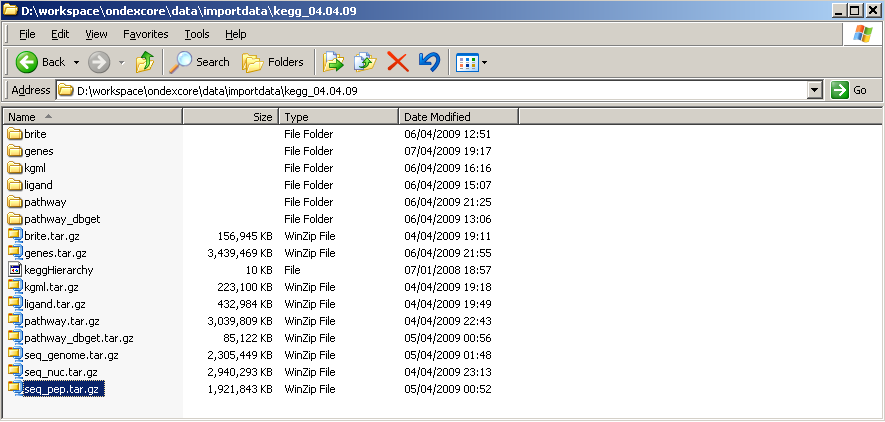
\includegraphics[scale=0.4]{images/Oct12/kegg_dir.png}
\caption{KEGG directory}
\label{fig:kegg_dir}
\end{figure}

\begin{itemize}
  \item{InputDir}\\
  Absolute path to input directory.
  \item{Species}\\
  This option provides a list of species to import pathways from KEGG for.
  Use ``all'' to include all available species.
  \item{ParseAllSequencesForSpecies}\\
  Specifies to parse all genes for a species regardless of membership of pathway.
  \item{SpeciesOrthologs}\\
  Parse orthologs to specified species
  \item{OnlyReferenced}\\
  Import only pathway entries which are referenced in relation or reaction section.
\end{itemize}
    
%%%%%%%%%%%%%%%%%%%%%%%%%%%%%%%%%%%%%%%%%%%%%%%%%%%%%%%%%%%%%%%%%%%%%%%%%%%%%%%%%%        
\section{KEGG parser, latest (Release 56.0, October 1, 2010)}
Parser for the KEGG database version 56 (\url{http://www.genome.jp/kegg/download/}). 
\begin{itemize}
  \item{InputDir}\\
  Absolute path to input directory.
  \item{Species}\\
  Specify the species code (NCBI taxID) of species to import pathways for.
  \item{ParseAllSequencesForSpecies}\\
  Specifies to parse all genes for a species regardless of membership of pathway.
  \item{SpeciesOrthologs}\\
  Parse orthologs to specified species.
  \item{OnlyReferenced}\\
  Import only pathway entries which are referenced in relation or reaction section.
\end{itemize}

%%%%%%%%%%%%%%%%%%%%%%%%%%%%%%%%%%%%%%%%%%%%%%%%%%%%%%%%%%%%%%%%%%%%%%%%%%%%%%%%%%        
\section{Medline/PubMed (MEDLINE 2011)}
Stable parser for MEDLINE (\url{http://www.nlm.nih.gov/bsd/pmresources.html}).
Parses any MEDLINE XML file. Use either PubMed to search for keywords and save results to XML or 
use Parser's integrated web-service functionality to fetch cited publications online.
\begin{itemize}
  \item{InputFile}\\
  Input file in PubMed/MEDLINE XML format.
  \item{ImportCitedPMIDs}\\
  Import publications that are cited in the Ondex graph. 
  Efetch web-service will be used to retrieve all information and new publication concepts will be created.
  \item{PubMedIdsFile}\\
  File which contains PubMed IDs to be parsed into Ondex (separated by line break). 
  Efetch web-service will be used to retrieve and create publication concepts.
\end{itemize}

%%%%%%%%%%%%%%%%%%%%%%%%%%%%%%%%%%%%%%%%%%%%%%%%%%%%%%%%%%%%%%%%%%%%%%%%%%%%%%%%%%        
\section{Medline parser (obsolete) (MEDLINE 2011)}
Second parser (experimental) for MEDLINE (\url{http://www.nlm.nih.gov/bsd/pmresources.html}) with different parameters. 
\begin{itemize}
  \item Summary \url{http://www.nlm.nih.gov/bsd/licensee/2009_stats/baseline_med_filecount.html}
  \item Download baseline: \url{ftp://ftp.nlm.nih.gov/nlmdata/.medleasebaseline/gz/}
  \item Download updates: \url{ftp://ftp.nlm.nih.gov/nlmdata/.medlease/gz/*.gz}
  \item reads files: PubMed export XML files, PMID files
  \item webservice: Efetch to get publications
\end{itemize}

All arguments are optional:
\begin{itemize}
  \item{Prefix}\\
  The Prefix letters that start the medline file in the form of "medline09n" where "09" is the year
  \item{Compression}\\
  The Compression file type currently on gunzip denoted by "gz" is permitted
  \item{PMIDInputList}\\
  List of PUBMED IDs separated by semicolon
  \item{XmlFiles}\\
  Medline XML files to include.
  \item{PubMedFile}\\
  Absolute path to an XML file which contains the results of a PubMed search, 
  {\it{e.g.}} search in PubMed for ``Arabidopsis'', click on ``Send to: '' at the top right-hand side of the PubMed page, 
  ``Choose destination'' and ``File'' to save the results.
  \item{ImportOnlyCitedPublications}\\
  Import only publications that are cited in the Ondex graph.
  \item{LowerXmlBoundary}\\
  The value of this argument is only taken into account if nothing is specified for PMIDInputList, XmlFiles, PubMedFile and ImportOnlyCitedPublications.
  In that case it will only parse Medline XML files which filename contains a number greater than this boundary.
  \item{UpperXmlBoundary}\\
  The value of this argument is only taken into account if nothing is specified for PMIDInputList, XmlFiles, PubMedFile and ImportOnlyCitedPublications.
  In that case it will only parse Medline XML files which filename contains a number lower than this boundary.
  \item{UseEfetchWebService}\\
  If set to true, uses NCBI's efetch to get publications. If false (default) parses local files.
  \item{InputDir}\\
  Absolute path to input directory.
\end{itemize}
    
    
%%%%%%%%%%%%%%%%%%%%%%%%%%%%%%%%%%%%%%%%%%%%%%%%%%%%%%%%%%%%%%%%%%%%%%%%%%%%%%%%%%        
%\section{Nodelist}
%Integrates a tab-delimited file that contains a list of nodes.
%\begin{itemize}
%\item{Id column}\\
%Specifies the number of the column that contains the node identifier.
%\item{Name column}\\
%Specifies the number of the column that contains the name.
%\item{Accession column}\\
%Specifies the number of the column that contains the accession data.
%\item{Source of accession}\\
%Specifies the source database that the accession stands for.
%\item{Concept class}\\
%Specifies the concept class that all nodes will be defined as.
%\item{Data source name}\\
%Specifies the name of the data source.
%\item{Input File}\\
%File with data to import.
%\end{itemize}
    
%%%%%%%%%%%%%%%%%%%%%%%%%%%%%%%%%%%%%%%%%%%%%%%%%%%%%%%%%%%%%%%%%%%%%%%%%%%%%%%%%%        
%\section{Nwb}
%Parser for the Network Workbench format.
%\begin{itemize}
%\item{Input File}\\
%File with data to import.
%\end{itemize}
    
%%%%%%%%%%%%%%%%%%%%%%%%%%%%%%%%%%%%%%%%%%%%%%%%%%%%%%%%%%%%%%%%%%%%%%%%%%%%%%%%%%    
\section{OMIM Parser}
Parser for the Online Mendelian Inheritance in Man (a database of human genes and genetic disorders).
Download from \url{http://www.ncbi.nlm.nih.gov/Omim/omimfaq.html#download}.
\begin{itemize}
  \item{InputDir}\\
  Absolute path to input directory. 
\end{itemize}
    
%%%%%%%%%%%%%%%%%%%%%%%%%%%%%%%%%%%%%%%%%%%%%%%%%%%%%%%%%%%%%%%%%%%%%%%%%%%%%%%%%%    
\section{OrthoXML (0.2)}
Parser for the OrthoXML format \url{http://orthoxml.org/}.
This format is used especially by Inparanoid \url{http://inparanoid.sbc.su.se/download/current/orthoXML/}.
\begin{itemize}
  \item{InputFile}\\
  Absolute path to an OrthoXML input file.
\end{itemize}   

%%%%%%%%%%%%%%%%%%%%%%%%%%%%%%%%%%%%%%%%%%%%%%%%%%%%%%%%%%%%%%%%%%%%%%%%%%%%%%%%%%    
\section{PDB flat file parser}
Protein Data Bank Parser. Download data from \url{ftp://ftp.wwpdb.org/pub/pdb/data/structures/all/pdb/}.
The Parser searches in a folder for all ``.enz-files'' and parses them.
\begin{itemize}
  \item{InputDir}\\
  Specifies the data directory.
  Can be used to define an absolute path, if the data is stored within the ondex data directory use the datadir parameter.
\end{itemize}
    
%%%%%%%%%%%%%%%%%%%%%%%%%%%%%%%%%%%%%%%%%%%%%%%%%%%%%%%%%%%%%%%%%%%%%%%%%%%%%%%%%%    
\section{Pfam}
Parser for the PFAM database, \url{http://pfam.sanger.ac.uk/}.
\begin{itemize}
  \item{SearchForPfam}\\
  When set to true, it just seaches for references.
  \item{InputFile}\\
  Absolute path to input file 
\end{itemize}
     
%%%%%%%%%%%%%%%%%%%%%%%%%%%%%%%%%%%%%%%%%%%%%%%%%%%%%%%%%%%%%%%%%%%%%%%%%%%%%%%%%%    
\section{Phytozome (7.0)}
Parser for any PHYTOZOME species.
This parser requires as input the annotation directory of a specific species. 
It parses the GFF3, peptide FASTA and CDS FASTA file inside of the annotation directory. 
It was tested on Arabidopsis, rice, poplar and brachypodium.
Requires files from annotation directories of parsed species: 
\url{ftp://ftp.jgi-psf.org/pub/JGI_data/phytozome/}
\begin{itemize}
  \item{InputDir}\\
  Path to a phytozome annotation directory for a given species ({\it{e.g.}}, phytozome/v7.0/Osativa/annotation/)
  \item{TaxID}\\
  Specify the NCBI/UniProt taxid of this species.
  \item{AccDataSource}\\
  Choose a data source for accessions ({\it{e.g.}}, TAIR (default: ENSEMBL)).
  \item{ChromosomeNumber}\\
  Enter the number of chromosomes for this species. 
  This is used to distinguish between main chromosomes and scaffolds (needed to use the Genomics layout after integration).
\end{itemize}
   
%%%%%%%%%%%%%%%%%%%%%%%%%%%%%%%%%%%%%%%%%%%%%%%%%%%%%%%%%%%%%%%%%%%%%%%%%%%%%%%%%%    
\section{PlnTFDB (2.0) parser}
PlnTFDB (2.0) is a public database \url{http://plntfdb.bio.uni-potsdam.de/v2.0/} arising from efforts to identify and catalogue
all Plant genes involved in transcriptional control. 
Download data from \url{http://plntfdb.bio.uni-potsdam.de/v3.0/downloads.php}.
The data from that site should be added to a directory (only the transcription factor list and protein sequence files are required).
\begin{itemize}
  \item{InputDir}\\
  Absolute path to input directory.
\end{itemize}
    
%%%%%%%%%%%%%%%%%%%%%%%%%%%%%%%%%%%%%%%%%%%%%%%%%%%%%%%%%%%%%%%%%%%%%%%%%%%%%%%%%%        
\section{Poplar Genome}
Parser for Poplar sequences and functional annotations.   
Files can be downloaded from: \url{http://genome.jgi-psf.org/Poptr1_1/Poptr1_1.download.ftp.html}.
\begin{itemize}
  \item{InputDir}\\
  Absolute path to input directory. 
\end{itemize}
  
%%%%%%%%%%%%%%%%%%%%%%%%%%%%%%%%%%%%%%%%%%%%%%%%%%%%%%%%%%%%%%%%%%%%%%%%%%%%%%%%%%        
\section{PSI-MI v2.5 stream parser}
Ondex parser for molecular interactions data. Aims to be compatible with all 
HUPO PSI-MI (Proteomics Standards Initiative - Molecular Interactions) 2.5 formatted files.
\begin{itemize}
  \item{InputFile}\\
  Absolute path to input file.
  \item{MappingFile}\\
  Location of the PSI-MI to Ondex mapping file
  \item{ParseSequences}\\
  Whether to parse contained DNA or AA sequences or not
  \item{InteractionTypeFallBack}\\
  Id of concept class to use for untyped interactions
\end{itemize}
    
%%%%%%%%%%%%%%%%%%%%%%%%%%%%%%%%%%%%%%%%%%%%%%%%%%%%%%%%%%%%%%%%%%%%%%%%%%%%%%%%%%        
\section{SBML Parser}
Systems Biology Markup Language (SBML) parser - not full functionality.
\begin{itemize}
  \item{InputFile}\\
  Absolute path to input file.. 
\end{itemize}
    
%%%%%%%%%%%%%%%%%%%%%%%%%%%%%%%%%%%%%%%%%%%%%%%%%%%%%%%%%%%%%%%%%%%%%%%%%%%%%%%%%%        
\section{SBML2 Parser}
Parser for Systems Biology Markup Language (SBML), using libSBML, targeting SBML level 2.
Install the 3.4 Xerces version of libSBML and modify runme.bat or runme.sh adding a parameter -Djava.library.path=``Path to SBML JAVA libraries''.
\begin{itemize}
  \item{InputDir}\\
  Directory with SBML files.
  \item{DataSource}\\
  ID of datasource (Ondex:DataSource) where the data has been obtained from.
\end{itemize}
    
%%%%%%%%%%%%%%%%%%%%%%%%%%%%%%%%%%%%%%%%%%%%%%%%%%%%%%%%%%%%%%%%%%%%%%%%%%%%%%%%%%        
\section{Tabular Parser}
Parses relations from tabular files.
\begin{itemize}
  \item{Skip}\\
  How many rows to skip at begin of document.
  \item{FromCol}\\
  Index of concept parser id for from concept.
  \item{ToCol}\\
  Index of concept parser id for to concept.
  \item{FromNameCol}\\
  ConceptName index for use with from concept.
  \item{ToNameCol}\\
  ConceptName index for use with to concept.
  \item{FromPhenoCol}\\
  Attribute Pheno index for use with from concept
  \item{ToPhenoCol}\\
  Attribute Pheno index for use with to concept.
  \item{ConfCol}\\
  Index of confidence score of relation.
  \item{TaxId}\\
  Which taxonomy id should be assigned to the sequences.
  \item{CC}\\
  The type of the concepts (e.g. target, gene, protein)
  \item{DataSource}\\
  The source of the concepts (e.g. TAIR, KEGG, unknown)
  \item{RelationType}\\
  The relation type to create for every line in the tabular file.
  \item{Threshold}\\
  Import threshold for confidence value.
  \item{FromTaxId}\\
  TaxID index for use with from concept.
  \item{ToTaxId}\\
  TaxID index for use with to concept.
  \item{InputFile}\\
  Delimited file to import.
\end{itemize}
    
%%%%%%%%%%%%%%%%%%%%%%%%%%%%%%%%%%%%%%%%%%%%%%%%%%%%%%%%%%%%%%%%%%%%%%%%%%%%%%%%%%        
\section{Table format parser}
\begin{itemize}
  \item{Sheet}\\
  If parsing data from an Excel spreadsheet this is a required argument.
  \item{Col\_separator}\\
  If parsing from a delimited file this is a required argument (Java regex).
  \item{FirstRow}\\
  First row (Optional).
  \item{LastRow}\\
  Last row (Optional for tab delimited files, strongly recomended for MS-EXCEL files).
  \item{Attribute}\\
  Convert value in the column into the specified property (attribute, name or accession), 
  the format is concept\_id,col,type,$[$type specific options$]$,
  where the first three argumetns are required and the rest are optional. 
  Type identifiers are (case insensitive): ATTRIBUTE, NAME or ACC. 
  Concept\_id can be anything and is just used to group the attributes to appropritate concepts. Examples:
  \begin{itemize}
    \item c1,1,NAME 
    \item c1,2,ACC,TAIR 
    \item c2,3,ATTRIBUTE,p-value,NUMBER 
    \item c2,4,ATTRIBUTE,description,TEXT 
    \item c3,5,ATTRIBUTE,count,INTEGER 
    \item c3,5,ATTRIBUTE,ChemicalStructure,SMILES 
  \end{itemize} 
  Optionally, you may append a regular expression string. 
  If it matches, the first group of such expression will be read as value. Example: c1,1,NAME,(.$\{2\}$).* will read the first two characters as name.
  \item{Concept\_class}\\
  Tuple of concept\_id and corresponding concept class it should have {\it{e.g.}}: c1,Protein
  \item{Data\_source}\\
  The source of the concepts (e.g. TAIR, KEGG, unknown)
  \item{InputFile}\\
  Table-like data representations file 
\end{itemize}
    
%%%%%%%%%%%%%%%%%%%%%%%%%%%%%%%%%%%%%%%%%%%%%%%%%%%%%%%%%%%%%%%%%%%%%%%%%%%%%%%%%%    
\section{TAIR (10)}

The hierarchy below describes both the structure of the required TAIR10 folder and subfolders, 
and where to download their content from (urls starting with ftp).

\begin{itemize}
\item{TAIR10}
	\begin{itemize}
	\item {\url{ftp://ftp.arabidopsis.org/Genes/TAIR10_genome_release/*}}
	\item {\url{ftp://ftp.arabidopsis.org/Proteins/Domain}}
	\item {\url{ftp://ftp.arabidopsis.org/Proteins/Id conversions}}
	\item {\url{ftp://ftp.arabidopsis.org/Sequences/blast_datasets/TAIR10_blastsets/TAIR10_pep_20101207}}
	\item {\url{ftp://ftp.arabidopsis.org/Sequences/blast_datasets/TAIR10_blastsets/TAIR10_cdna_20101207}}
	\item {\url{ftp://ftp.arabidopsis.org/home/tair/Genes/TAIR10_genome_release/TAIR10_locushistory.txt}} 
	\end{itemize}
\end{itemize}
The two parameters for this parser are as follows:
\begin{itemize}
  \item{Annotation}\\
  If set to true, publications (LocusPublished file), protein domain information 
  and UniProt accessions (rather than just the FASTA sequence files) will also be parsed in.
  \item{InputDir}\\
  Absolute path to input directory. 
\end{itemize}
    
%%%%%%%%%%%%%%%%%%%%%%%%%%%%%%%%%%%%%%%%%%%%%%%%%%%%%%%%%%%%%%%%%%%%%%%%%%%%%%%%%%    
\section{NCBI Taxonomy Parser}
Parser for the NCBI Taxonomy database. Creates a is\_a hierarchy of terms. Uses names.dmp and nodes.dmp.
\begin{itemize}
  \item{Root}\\
  At which root node in taxonomy tree should the parser start. Any valid taxonomy id.
  \item{InputDir}\\
  Directory with taxonomy files. 
\end{itemize}
    
    
%%%%%%%%%%%%%%%%%%%%%%%%%%%%%%%%%%%%%%%%%%%%%%%%%%%%%%%%%%%%%%%%%%%%%%%%%%%%%%%%%%    
%\section{Timeseries}
%\begin{itemize}
%\item{TAXID}\\
%NCBI TaxID
%\item{ConceptClass}\\
%ConceptClass to map probes/targets to
%\item{IgnoreLSD}\\
%Ignore the Least Significant Difference restrictions
%\item{IsRatio}\\
%Data is a ratio to t0
%\item{Input File}\\
%File with data to import.
%\end{itemize}
    
%%%%%%%%%%%%%%%%%%%%%%%%%%%%%%%%%%%%%%%%%%%%%%%%%%%%%%%%%%%%%%%%%%%%%%%%%%%%%%%%%%    
\section{Transfac parser}
Parses the Transfac database from BioBase (\url{http://www.gene-regulation.com/pub/databases.html}).
\begin{itemize}
  \item{InputDir}\\
  Absolute path to input directory.
\end{itemize}
    
%%%%%%%%%%%%%%%%%%%%%%%%%%%%%%%%%%%%%%%%%%%%%%%%%%%%%%%%%%%%%%%%%%%%%%%%%%%%%%%%%%    
\section{Transpath parser}
Parses the Transpath database from BioBase (\url{http://www.gene-regulation.com/pub/databases.html}).
\begin{itemize}
  \item{ParseMolecules}\\
  ParseMolecules
  \item{ParsePathways}\\
  ParsePathways
  \item{InputDir}\\
  Absolute path to input directory. 
\end{itemize}
    
%%%%%%%%%%%%%%%%%%%%%%%%%%%%%%%%%%%%%%%%%%%%%%%%%%%%%%%%%%%%%%%%%%%%%%%%%%%%%%%%%%    
\section{UniProt (UniProt release 2011.06)}
Parser for the UniProt Knowledgebase database (\url{http://www.uniprot.org/downloads}, download in XML format). 
Implements this \url{http://www.devx.com/Java/Article/30298/0/page/2} way of parsing a xml file.

\begin{itemize}
  \item{InputFile}\\
  UniProt XML file 
  \item{TaxId}\\
  Only parse proteins with exactly this taxonomy id
  \item{GoFile}\\
  GO OBO file. This will link proteins with proper GO concepts of ConcepClass MolFunc, BioProc and CelComp. 
  If not specified GO accessions are part of proteins.
  \item{DbRefAcc}\\
  If set to true, will search for accessions which already belong to a concept in the given graph
  \item{Accessions}\\
  A list of comma separated accession numbers (any acc, does not need to be uniprot acc), which should be parsed from the given uniprot file
  \item{AccessionsFile}\\
  Path to the file containing a list of accession numbers (one acc per every line), which should be parsed from the given uniprot file	
  \item{TagInformation}\\
  If set to true, will attach tag information to the concepts
  \item{HideLargeScaleRef}\\
  If set to true, will hide large scale references (publications)
\end{itemize}

%%%%%%%%%%%%%%%%%%%%%%%%%%%%%%%%%%%%%%%%%%%%%%%%%%%%%%%%%%%%%%%%%%%%%%%%%%%%%%%%%%    
\section{Wordnet}
Works only with most recent Windows version of WordNet 2.1.
Download from \url{http://wordnet.princeton.edu/wordnet/download/#win}
Put data.adv, data.verb, data.adj, data.noun into data/importdata/wordnet or folder to be parsed.
\begin{itemize}
  \item{InputDir}\\
  Absolute path to input directory.  
\end{itemize}
